\documentclass[11pt,letter]{article}
\usepackage[top=1.00in, bottom=1.0in, left=1.1in, right=1.1in]{geometry}
\renewcommand{\baselinestretch}{1.1}
\usepackage{graphicx}
\usepackage{natbib}
\usepackage{amsmath}
\usepackage{textcomp}
\usepackage[
singlelinecheck=false % <-- important
]{caption}
\usepackage{float}
\usepackage{hyperref}

\def\labelitemi{--}
\parindent=0pt



\begin{document}
\bibliographystyle{/Users/Lizzie/Documents/EndnoteRelated/Bibtex/styles/besjournals}
\renewcommand{\refname}{\CHead{}}

\title{Safety plan for Wolkovich Lab: Okanagan field work}
\date{\today}
% \author{}
\maketitle
\tableofcontents

\section{General overview}
This research involves a small crew of two or three people visiting vineyards in the Okanagan valley to establish a phenology monitoring project that will run for at least a more two years. The Okanagan valley is not remote and the vineyards are all closely managed, so risk to fieldworkers is generally low. Potential hazards include walking over uneven ground, carrying equipment, exposure to cold and heat, and interactions with wildlife. There are also hazards associated with travel to and from field sites. In addition, the current COVID-19 situation creates additional hazards for both field workers and local communities, but we deem these risks to be low and are taking appropriate action as recommended by WorkSafe BC \url{https://www.worksafebc.com/en/about-us/covid-19-updates/covid-19-industry-information/forestry}. 

\section{Personnel and Contact Information}

\subsection {Field Crew}

There will be a main team of two field operatives (Faith Jones and Mira Garner) for the full three week period. Additionally, Lizzie Wolkovich and her partner Jonathan Davies will be present for the first week (longer if there are any safety concerns or issues).  Jones and Garner will travel up in one UBC vehicle, and Wolkovich with Davies in their personal vehicle (BC plate FP254E). Wolkovich and Davies will also stay at a different location than Jones and Garner, although both locations will be within 10 km from Penticton.   

\subsection {Contact Details}

\begin{table}[H]
\caption{Field crew contact details} % title of Table
%\centering % used for centering table. I dont want my tabel centred 
\begin{tabular}{ l | l }  % left jusitfy columns (2 columns)
\hline\hline %inserts double horizontal lines
Name & Contact\\ [0.5ex] % inserts table
%heading
\hline % inserts single horizontal line
Elizabeth Wolkovich & 603 667 5099\\ % inserting body of the table
Faith Jones & 604 786 2574 \\
Mira Garner & 608 228 5215 \\
Jonathan Davies & 604 822 5486 \\ 
\hline %inserts single line
\end{tabular}
\label{table:nonlin} % is used to refer this table in the text
\end{table}

\begin{table}[H]
\caption{Field crew emergency contact details} % title of Table
%\centering % used for centering table
\begin{tabular}{l l l} % left jusitfy columns (3 columns)
\hline\hline %inserts double horizontal lines
Field Crew Member & Name & Contact\\ [0.5ex] % inserts table
%heading
\hline % inserts single horizontal line
Elizabeth Wolkovich & Jeanne Dearden (mother) & 603 236 9370 \\ % inserting body of the table
Faith Jones & Peter Walton (spouse) & 604 803 0664\\
Mira Garner & Hiam Garner (father) & 608 576 5215 \\
Jonathan Davies & Pedro Peres-Neto & 514 825 5579\\
\hline %inserts single line
\end{tabular}
\label{table:nonlin} % is used to refer this table in the text
\end{table}

\begin{table}[H]
\caption{Other contact details} % title of Table
%\centering % used for centering table
\begin{tabular}{l l} % left jusitfy columns (3 columns)
\hline\hline %inserts double horizontal lines
Name & Contact \\ [0.5ex] % inserts table
%heading
\hline % inserts single horizontal line
General Emergencies & 911 \\ % inserting body of the table
Kelowna General Hospital & 250 862 4000 \\
Pat Bowen & 250 494 6424\\
Carl Bogdanoff & 250 490 9710 \\ % gave their home phone here, Carl's cell 250 809 7738
Quails Gate vineyard main office & 250 769 4451 \\
Arterra vineyard main office & 250 498 4981\\ % (250) 498-9391 cell for Mike Watson

\hline %inserts single line
\end{tabular}
\label{table:nonlin} % is used to refer this table in the text
\end{table}

\subsection {Nearest Hospitals}
Penticton Regional Hospital \newline
550 Carmi Avenue\newline
Penticton, BC V2A 3G6\newline
Phone: 250-492-4000\newline
Open for emergencies 24/7\newline

Kelowna General Hospital\newline
2268 Pandosy Street\newline
Kelowna, BC V1Y 1T2\newline
Phone: 250-862-4000\newline
Open for emergencies 24/7\newline

Vernon Jubilee Hospital\newline
2101 - 32nd Street\newline
Vernon, BC V1T 5L2\newline
Phone: 250-545-2211\newline
Open for emergencies 24/7\newline

\subsection {General Safety Items}

\subsubsection{Overview}
\begin{figure}
  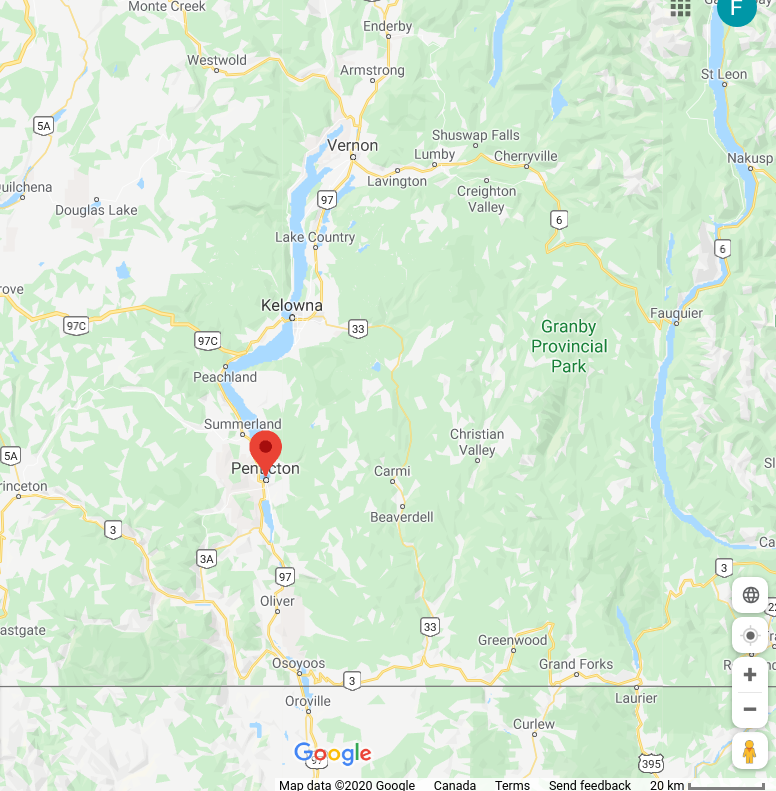
\includegraphics[width=\linewidth]{penticton.png}
  \caption{A map of the Okanagan Valley showing the location of Penticton, where the field crew will be based. Work will take place in the Valley from approximately Peachland to Oliver.}
  \label{fig:OkanMap}
\end{figure}
The field crew will be based in Penticton (49.481024, -119.587796; Figure\ref{fig:OkanMap}). Fieldwork will involve driving to various vineyards within a 30 km around the Okanagan valley. All sites are accessible by well maintained roads. Once on site, crew members will review vineyard locations for sampling (in consultation with Bowen and Bogdanoff and using maps provided by them) to plan which vines will be selected for phenological monitoring next year. This activity needs to take place this year because our contacts with the vineyards are retiring this year and so will be unavailable to facilitate project set up next year. This is also a critical time of year to view the buds and canes for selection, and because later in the year the vineyard employees are applying various management regimes in the vineyards. Working now is thus best for the research and most reduces the chances of coming into contact with vineyard employees.   

\subsubsection{Equipment and training}
Vehicles have been recently serviced and contain a first aid kit. A printed copy of the lab emergency procedure, emergency contacts, MSP information, and the location of the nearest hospital or clinic will also be stored with the field safety equipment. Crew members will work in pairs, while practicing appropriate social distancing measures. They will also carry mobile phones with them, as mobile phone reception is not problematic in the Okanagan Valley, and the first aid kits will be easily accessible in the vehicles on site. All vehicles used for fieldwork will be properly maintained and include equipment such as jumper cables, a fire extinguisher, and a spare tire. To avoid fatigue, no driver will drive for long periods without breaks. All drivers have more than 5 years of experience. All individuals will wear appropriate clothing and have access to sunscreen and insect repellent. Workers will also carry ample food and water to avoid fatigue and dehydration.  


\section{Identifying and Addressing Specific Health and Safety Concerns}

\subsection{COVID-19}

We are following the principles and guidelines laid out by WorkSafe BC specifically for Forestry and Agriculture field work and COVID-19 safety \url{https://www.worksafebc.com/en/about-us/covid-19-updates/covid-19-industry-information/forestry}. 

\subsubsection{Overview}
The crew consists of three active field members plus an additional driver who will not be in the field. This additional driver is Wolkovich's partner Jonathan Davies, who will be available to share driving with Wolkovich but will not undertake active field duties in vineyards. Other than driving to and from the accommodation, and driving to the field sites, all of the work is outdoors, and there will be no difficulty in maintaining appropriate social distancing of two meter minimum distances. Any team meetings will take place outside to maintain physical distance. All team members will be responsible for ensuring physical distancing is maintained and any special COVID-19 precautions are strictly followed as per WorkSafe BC guidelines. Good hygiene will be practiced at all times, in line with the  WorkSafe BC recommendations. 

\subsubsection{Location}
Jones and Garner will stay in a large apartment near Penticton. They will have separate bedrooms and washrooms, and will sanitize communal space and equipment regularly and remain 2 meters apart at all times. Wolkovich and Davies will stay in a separate apartment close by, but will not need to maintain social distance as they are already isolating as a family unit. \\

Each crew member will have their own sanitizer and hygiene supplies for personal use for the duration of the field work. There will also be bulk liquid soap, water, and sanitizer that the crew can use to fill their personal containers if the need arises.

\subsubsection {Travel}
Lizzie will be in her own vehicle along with her partner Jonathan, while Jones and Garner will share a field vehicle. Lizzie and Jonathan are already isolating as a family unit so do not need to maintain social isolation from each other. In the vehicle shared by Jones and Garner the passenger will sit in the back-passenger seat, diagonally positioned relative to the driver to maintain a two meter distance ensuring physical distancing is in place as per WorkSafe BC guidelines. All crew will wash hands with soap and water (or with hand sanitizer) prior to entering the vehicles. The interior (e.g. seatbelts, headrests, door handles, steering wheels, and hand holds) and exterior door handles of both vehicles will be wiped down with sanitizing cleaner at the end of each day, or sooner if a member of the crew reports COVID-19 symptoms.

\subsubsection {Tracking health before, during and after field work}
Only healthy team members will be allowed to travel. Any crew member that has had a confirmed case of COVID-19 or who is unwell at the time of departure based, will not be allowed to take part in this research project. During field work and for two weeks after crew members will monitor closely for symptoms and maintain a record of daily personal temperatures. Temperature screening will be done with a properly calibrated thermometer, with temperature thresholds based on Health Canada guidelines. An indicator for possible COVID-19 infection is 37.5 $^{\circ}$C. Active daily monitoring will be conducted using the Personal Health Daily Monitoring Form (from the BC Center for Disease Control), provided as an appendix (``COVID19-Contact-monitoring-form.pdf'').

\subsubsection{Exhibiting COVID-19 symptoms}
If a crew member exhibits COVID-19 symptoms (e.g. sore throat, fever, sneezing or coughing) they would be put into the far back seat of their truck, and instructed to put on a protective face mask and gloves. The other crew member of the pair, if not already the driver, would become the driver and they would put on a protective face mask and gloves. The inside of the vehicle (e.g. seatbelts, headrests, door handles, steering wheels, and hand holds) would then be wiped down with sanitizing cleaner. The vehicle would immediately head back to Vancouver not stopping along the way (there will be extra food/water in SUV). The drive time would be up to but likely not more than 6 hours. During the drive, the person with symptoms would continue to monitor their situation using a thermometer and tracking other health metrics (see Personal Health Daily Monitoring Form provided as an appendix). The field crew have thermometers in the vehicles to enable effective monitoring. The vehicle interior and exterior door handles would be wiped down with sanitizing cleaner upon completion of the drive. Following the protocols set out by WorkSafe BC, both the person with symptoms and the driver would go into self-isolation in their homes for two weeks. The research supervisor would immediately notify the Public Health Authority in British Columbia by dialing 811 that someone with symptoms is self-isolating. We would notify the management of our field accommodation so that they could take necessary cleaning precautions.  Any crew that has had a confirmed case of COVID-19 will not be allowed to come to work.

\subsubsection{Interactions with collaborators}
The field crew will need some interaction with local collaborators, but will maintain social distance from then as per the WorkSafe BC recommendations. To this end, all meetings will be kept to a minimum, and will take place outside where there is enough space for 2 meters between every person. The field crew will also practice good hygiene, including wearing face masks, not touching faces, washing hands often and for at least 20 seconds (or sanitizing hands if washing not possible) and sneezing/coughing into disposable tissues if needed.  

\subsubsection{Interactions with field workers in vineyards}
The field crew will alert vineyards to our presence on site so the field crew and vineyard field workers will be aware of each other's presence. Our fieldwork does not require interaction with such workers, so if the field crew see any workers they will retreat to a safe distance until they have left the immediate area. Any surfaces the field crew and vineyard fieldworkers might come into contact with will be sanitized before and after contact. Our crew members will also maintain a 2 meter distance from each other at all times as per the WorkSafe BC guidelines.   

\subsubsection{Interactions with local communities}
The field base will be close to the town of Penticton, where the field crew will obtain necessary groceries and gas. To reduce risk to local communities, shopping trips will be kept to a minimum (once a week), during shopping researchers will wear face masks, and sanitize hands before and after shopping, and maintain good hygiene. The field crew will only use self-service gas stations and prior to use we will wipe down the gas pump nozzle and PIN pad on the pump with sanitizing wipes. The field crew will not come into contact with any First Nation communities in the Okanagan Valley. 


\end{document}

The fieldwork in the Okanagan should be OK as long as your crew is small, there are no more than two people in a vehicle together, one driving and one in the back right seat (unless from the same household), social distancing can be maintained while working and in accommodations (unless from the same household), and there is no contact with indigenous communities. I've attached a few exemptions that have been approved, and here's a useful link to the WorkSafe BC recommended safety practices for forestry fieldwork that has largely been adopted by some of the other applications (Simard and Hinch). https://www.worksafebc.com/en/about-us/covid-19-updates/covid-19-industry-information/forestry I know working in a vineyard and in a remote field site are different, but there are still transportation, social distancing, PPE and sanitation concerns. You will also need to address how you will interact with or avoid farm workers at these sites. I would also say that you should be able to get the plots set up, but should defer any data collection that can wait for next year.

Need:
face masks for everyone
thermometers maybe?
hand sanitiser and cleaning stuff (Faith has one bottle of hand sanitiser)
gloves x 3 at least 

Questions:

Does Johnathan need including in the plan, at least re being able to dive Lizzie home if she gets sick?
